\begin{frame}
   {uSD card}
   \begin{figure}[H]
      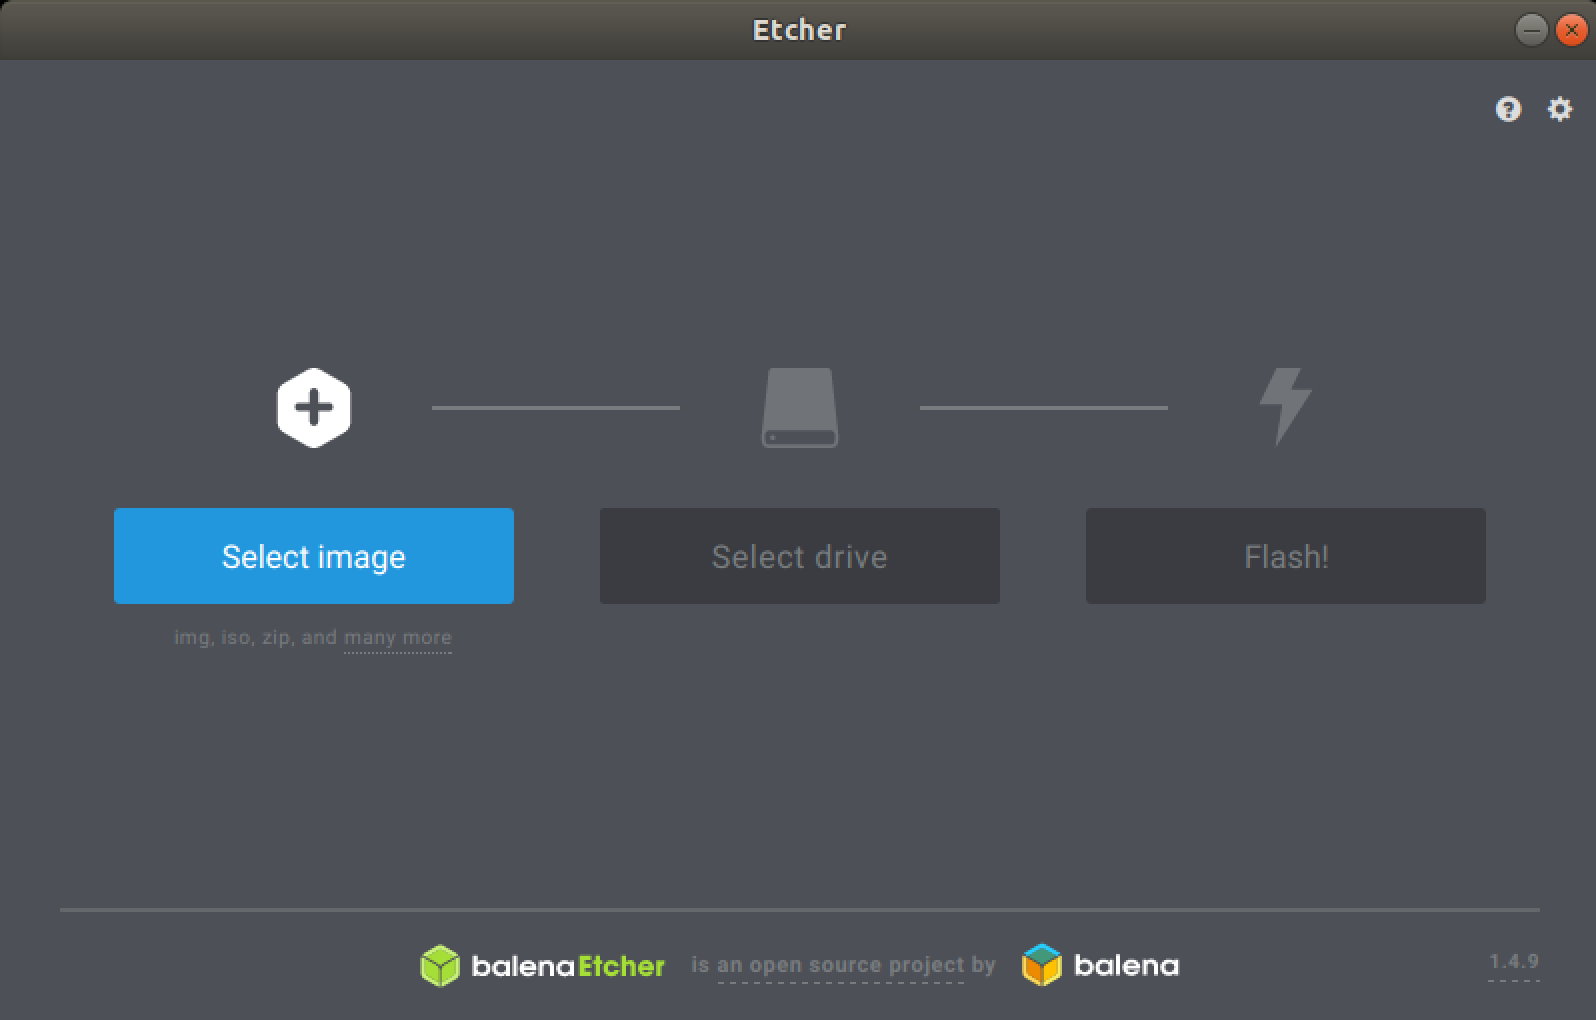
\includegraphics[height=2in]{IMAGES/balene-etcher}
   \end{figure}
   \begin{itemize}
      \item We will install a Raspbian image directly (instead of using NOOBS)
	      to the uSD card with \textbf{Balena Etcher}
      \item This will allow us to setup our board over a USB cable
   \end{itemize}
\end{frame}

\cprotect\note{

   Once the burn is complete you will need to pull the sd card out then
   reinsert it into the card reader to have it automounted under \verb?/media/$USER?

   Once mounted we have to make a few changes to the files on the next page.

}

